\chapter{概率与统计 - 数学期望、统计描述 \& 分布}

\begin{figure}[ht]
  \centering
  
\includegraphics[width=1\textwidth]{asset/20230917201549.png}
\end{figure}
\newpage


在上一节中, 我们最后有谈到随机变量. 在概率论几统计学中, 描述一个随机变量的离散程度的有方差、标准差等等. 那么在这节课中, 我们就来好好看看这些概念. 

不过在这之前呢, 我们先来看看什么是「数学期望」. 

\section{数学期望}

数学期望告诉我们, 对于随机试验的结果, 我们可以有怎样定量的期待. 

也就是说, 实验还没做之前, 可以有怎么样的一个期待. 这个也就是数学期望这个词的一个来源. 

比如我们上赌桌了, 去赌有两种结果, 第一种结果就是赚的盆满钵满, 回报1,000美刀, 但是概率只有$0.001$. 第二种情况是你的赌资50刀没了, 这个发生的概率是非常非常高, 有$0.999$, 也就是$99.9\%$. 

\begin{figure}[ht]
  \centering
  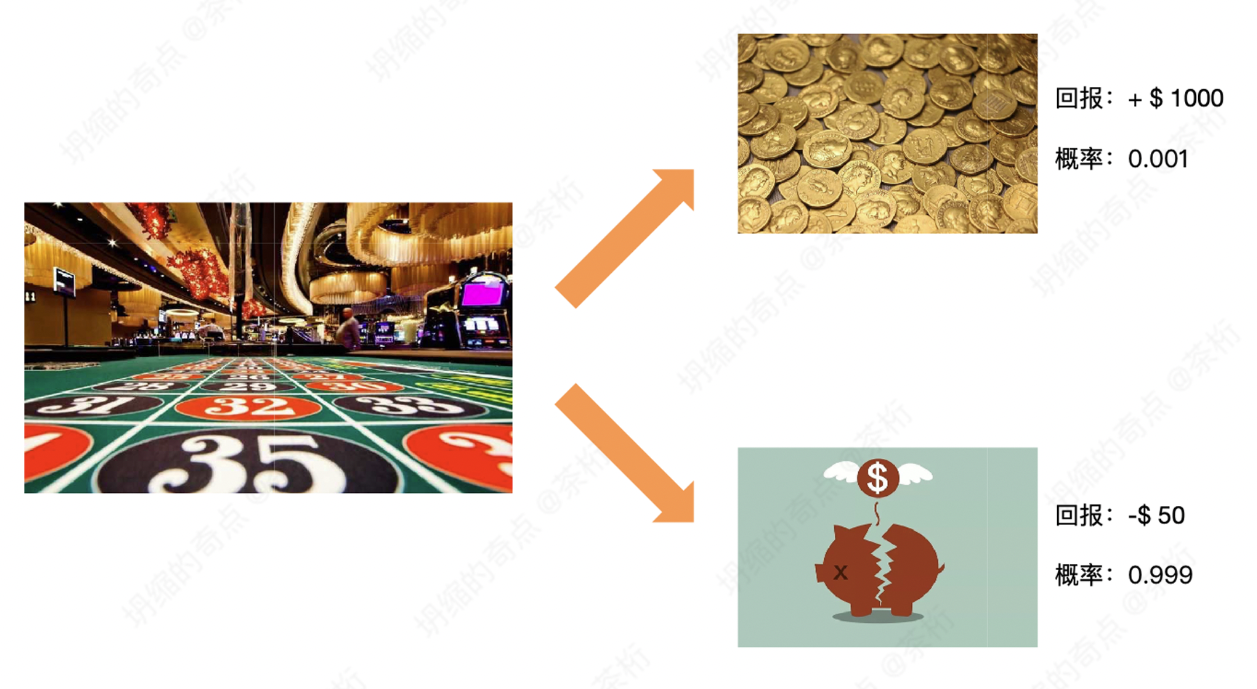
\includegraphics[width=0.9\textwidth]{asset/20230826212939.png}
  \caption{}
  \label{fig:img22_1}
\end{figure}

那我们在赌之前, 怎样预估一下这一次事件干了之后, 会得到一个怎样的结果呢?这时候, 数学期望就发挥作用了. 数学期望的方式就是把每种可能的结果乘上对应的概率, 然后再相加. 

我们在进行大量试验之后, 看到自己能够收到的平均回报是多少?

\begin{align*}
  E(X) = 1000 \times 0.001 + (-50) \times 0.999 = -48.95
\end{align*}

大量进行实验, 平均每一回合我们的这个回报是倒贴48块9毛5, 所以这个就得慎重了. 

数学期望不止可以让我们去做一些预测性的判断, 同样呢还可以帮我们去解决一些分配性的事情, 比如说有两个人赌博, 对于每一局而言他们两个获胜的几率都是相等的. 比赛是五局三胜, 赢家可以拿到100刀. 

第四局开始前, 因为一些特殊情况, 比赛不能继续下去了. 前三局甲已经赢了两局, 已已经赢了一局, 现在的问题是在没办法继续进行比赛的前提下, 我们该如何公平的分配这100刀?

这道题我们之前导论课上其实已经做过了, 现在让我们就简短过一下. 我们怎么样去分析呢?比赛没比完, 怎么样去去判断给谁多少钱呢?剩下的比赛如果继续的话, 甲的赢面是有多大, 乙赢面有多大, 也就是他们最终获胜的概率是多大. 这个就是我们的一些分析. 

比赛继续, 甲再赢一局就获胜了, 乙需要两场全赢. 所以, 甲不获胜, 点背两场都输了, 所以概率1/4. 

甲最终不获胜的概率: $P(\mbox{甲负})= 1/2 \times 1/2 = 1/4$

反面就是甲获胜, 拿1去减就是3/4: $P(\mbox{甲胜}) = 1 - P(\mbox{甲负}) = 3/4. $

同样的情况对于乙而言也是这样, 他最终获胜必须两局都赢下来, 所以是概率1/4: $P(\mbox{乙胜})  = 1/2 \times 1/2 = 1/4$. 

他最终不获胜就是3/4:  $P(\mbox{乙负}) = 1 - P(\mbox{乙胜})  = 3/4$. 

所以, 按照甲可获得的奖金这个期望值是多少, 获胜给你多少钱. 实际上获胜的概率3/4, 不获胜回报0, 不获胜的概率有1/4, 得出来是75: $E(\mbox{甲}) = 100 \times 3/4 + 0 \times 1/4 = 75$;

乙呢同样通过计算呢是25: $E(\mbox{乙}) = 100 \times 1/4 + 0 \times 3/4 = 25$;

通过这种方式, 我们就能公平的把这100刀给甲和乙分掉. 甲拿75刀, 乙拿到25刀. 

因为在我们设想比赛继续进行的情况下, 甲获得奖金的期望值就是75, 乙就是25. 

但是在这里有一点大家需要注意一下, 这样做有可能不一定公平. 比如说实际情况里面乙可能后来居上, 可能后来的状态比较好, 甲可能后来状态不行. 最终我们按照这种模型去预测的结果就是不准确的. 但是为什么我们依然按照这种方式去做奖金的分配呢?因为你不按照这种方式去做你拿啥去做?所以这是我们唯一可选择的一个路子了. 

就跟好多人说那个高考不公平一样, 那如果高考不公平那你觉得啥公平呢?高考的时候只看分数, 跟你的出身家境什么都没有任何关系, 所以如果高考不公平, 那还有比他更公平的事情吗?

我们再来看一下数学期望的一些性质, 我就不给大家一条一条去说了, 这个以前我们也上过. 大家回过头来复习的时候把这个看一下就好了. 

\begin{enumerate}
  \item $EC = C$, $C$为常数
  \item $E(CX) = CE(X)$, $C$为常数
  \item $E(X + Y) = E(X) + E(Y)$
  \item $E(XY) = E(X)E(Y)$, 当$X,Y$相互独立时
  \item $E(XY)$需按照定义去计算, 当$X,Y$不独立时
\end{enumerate}

\section{方差}

我们还是直接用例子来解释方差, 当我们投掷一枚骰子, 其向上的点数期望值为: 

\begin{align*}
  E(\mbox{点数})  = 1/6 \times 1 + 1/6 \times 2 + 1/6 \times 3 + 1/6 \times 4 + 1/6 \times 5 + 1/6 \times 6 = 3.5
\end{align*}

但是, 3.5并不代表着什么, 朝上点数要么是3要么是4. 我们知道实际情况各个点数出现的次数都是均等的, 所以在这种情况下我们还需要另外一个量去描述概率模型这些随机事件. 如何刻画这种差异?这就对应了方差, 方差代表了随机变量和期望之间的一个偏离程度. 

在这种情况下, 因为各个点数出现的次数都相等, 所以当朝上的点数是3和4的时候, 他和期望的差值比较少. 但如果是1或者6、又或者2和5的时候, 这个差值是比较大的. 所以我们就通过这个来描述随机变量可能取值, 离数学期望的一个偏离程度. 方差标准定义为: \textbf{「度量随机变量和其数学期望之间的偏离程度」}: 

\begin{align*}
  D = \sigma ^ 2 = \sum_{i=1}^N \frac{(X-E(X))^2}{N}
\end{align*}

就比如说, 有A, B两个人工智能模型, 它们在一系列同分布的数据集上的分类精确率如表\ref{tab:table22_1}所示, 试判断哪个模型表现更好. 

\begin{table}[ht]
  \centering
  \begin{tabular}{lllllll}
    \midrule
      A & $90\%$ & $92\%$ & $93\%$ & $91\%$ & $92\%$ & $94\%$  \\
      B & $88\%$ & $97\%$ & $90\%$ & $96\%$ & $94\%$ & $87\%$  \\
    \bottomrule
  \end{tabular}
  \caption{}
  \label{tab:table22_1}
\end{table}

那就让我们先来计算一下均值看看: 

\begin{align*}
  E(A) = \frac{90\% + 92\% + 93\% + 91\% + 92\% + 94\%}{6} = 92\% \\
  E(B) = \frac{88\% + 97\% + 90\% + 96\% + 94\% + 87\%}{6} = 92\% 
\end{align*}

如果是从均值判断的话, 我们会发现A、B两个模型都是一样, 识别准确率都是92\%. 问题是我们就能说这两个没有区别的吗?当然不是. 

方差判断可以通过这个方差的公式分别把它们计算出来: 

\begin{align*}
  \sigma^2(A) & = \frac{(0.9-0.92)^2+(0.92-0.92)^2+(0.93-0.92)^2}{6} \\ & + \frac{(0.91-0.92)^2+(0.92-0.92)^2+(0.94-0.92)^2}{6} \\ & = 0.000167 \\ \\
  \sigma^2(B) & = \frac{(0.88-0.92)^2+(0.97-0.92)^2+(0.90-0.92)^2}{6} \\ & + \frac{(0.96-0.92)^2+(0.94-0.92)^2+(0.87-0.92)^2}{6} \\ & = 0.0015 \\ \\
  & \sigma^2(A) < \sigma^2(B) \\
\end{align*}

我们可以发现, A的方差比B的方差要小, 方差小意味着随机变量波动情况会比较小, 它的这个曲值在期望的附近是比较稳定的. 所以模型A的表现更稳定, 我们说它的这个表现更好. 

那为什么我们要把这个方差做一个平方的处理呢?

\[
  \sigma ^2= \sum_{i=1}{N}\frac{(X-E(X))^2}{N} \quad ??
\]

我们不平方不行吗?

\[
  \sigma = \sum_{i=1}{N}\frac{(X-E(X))}{N}\quad ??
\]

确实是不行的, 因为如果不平方的话, 正负相消了, 方差按照定义计算出来就是0了, 如图\ref{fig:img22_2}. 

\begin{align*}
  \frac{(+6)+(+6)+(-6)+(-6)}{4} = 0
\end{align*}

\begin{figure}[ht]
  \centering
  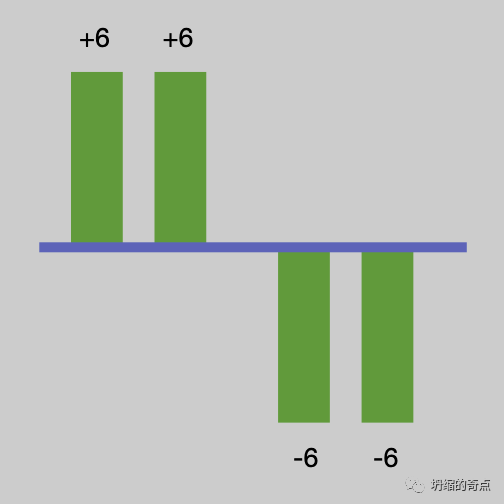
\includegraphics[width=0.5\textwidth]{asset/snap2023-12-29_02.10.20.png}
  \caption{}
  \label{fig:img22_2}
\end{figure}

很显然, 图中四个数据点彼此之间不是说没有相互偏离的, 相反上方两个数据点和下方两个数据点之间相差能到12个单位. 所以为了避免这个问题我们用一平方. 当然如果用绝对值也OK, 但是绝对值有一个天然不好的地方, 就是它在数学运算当中不太好去除. 绝对值要去除的话, 得关心他什么时候取正, 什么时候取负. 所以我们统一的就用平方来处理. 

\section{标准差}

标准差是什么概念呢?标准差其实很简单, 就是把方差开个平方就行了. 

\begin{align*}
  \sigma = \sqrt{\sum_{i=1}^N \frac{(X-E(X))^2}{N}}
\end{align*}

它的度量的效果其实和方差是一样的. 

哎, 一个新概念, 什么叫度量效果和方差一样?就是说方差能反映出来随机变量取值的偏离情况怎么样, 标准差同样可以. 如果方差大, 标准差就是做一个开方, 肯定也大. 

但是标准差为什么还要被设计出来? 因为方差有个平方,如果我们所统计的东西有一个很明确的物理含义,那方差的量纲就和随机变量不一致了. 不一致的话往往就会有一些问题. 比如我们如果要去做一些数据归一化, 除以方差就不太好去做. 

量纲其实就是单位, 量纲单位对不上的话, 两个数加减乘除就不太好做. 所以我们也有需要用到标准差的这个情景. 

方差的一些相关性质就列在这里, 不一一跟大家详细讲解了: 

\begin{enumerate}
  \item $D(C) = 0$, $C$为常数
  \item $D(X+C) = D(X)$, $C$为常数
  \item $D(CX) = C^2 D(X)$, $C$为常数
  \item $D(X+Y) = D(X) + D(Y) + 2Cov(X, Y)$
  \item $D(X+Y) = D(X) + D(Y)$ , 当X和Y相互独立时 
\end{enumerate}

$Cov(X,Y)=E{[X-E(X)][Y-E(Y)]}$:协方差

但是这里会涉及到一个新概念, 就是协方差. 

\section{协方差}

这个协方差是干嘛的呢?它跟方差是一字之差, 它是用于衡量两个变量的一个总体误差. 这句话如果单纯我们去看, 感觉get不到任何点, 那么就看下面这两句话: 

如果协方差为正, 代表这两个变量的变化趋势相同, 当一个大于其期望值时, 另一个也大于, 小于的情况亦然. 

打个比方, 两个高中生是同桌, 我们认为他们学习习惯会相互影响, 如果A的学习成绩提高, 那B也提高. 这个时候A、B他们俩的成绩所对应的这个斜方差为正. 如果一个成绩变差了, 因为他们学习习惯相互影响, 另外一个也受到影响, 成绩也差了. 

所以当一个随机变量大于它的期望值的时候, 另外一个随机变量也会大于期望. 如果小于也是一样. 

协方差为负, 代表着两个变量变化的趋势相反, 当一个大于其期望值时, 另一个就小于, 反之亦然. 

比如班上有两个非常厉害的人争夺班上的第一名, 这一次要么A考第一, B就得第二. 要么B考上第一, A就得第二. 他们俩此消彼长, 变化趋势相反, 你上去了我就下来, 咱们现在单纯是看排名. 

协方差出了为正或者为负, 还有一个特殊的情况, 就是协方差为0. 这个时候, 两个变量就没有线性相关性了. 也就是协方差其实反映的是一种线性相关性. 

如果两个变量是独立的, 独立的就代表它们不光没有线性相关性, 非线性的相关性也没有. 这个时候, 协方差是一定为0的. 可是反之并不一定成立. 也许它俩是一种非线性的一种相关性, 比如说$y=x^2$. 

协方差也是有公式的,下面是一些推导: 

\begin{align*}
  & Cov(X,Y)=E\{[X - E(X)][Y - E(Y)]\} \\
  & = E\{XY-XE(Y)-YE(X)+E(X)E(Y)\} \\
  & = E(XY)-E[XE(Y)]-E[YE(X)]+E(X)E(Y) \\
  & = E(XY)-E(X)E(Y)-E(X)E(Y)+E(X)E(Y) \\
  & = E(XY)-E(X)E(Y)
\end{align*}

当X,Y独立时, $E(XY)-E(X)E(Y) = 0 \Rightarrow Cov(X,Y) = 0$

在这里就不说了, 导论课都说过. 咱们把这个简单的例子再看一遍吧, 我们先来看表\ref{tab:table22_2}: 

\begin{table}[ht]
  \centering
  \begin{tabular}{lllllll}
    \midrule
      数学 & 90   & 92   & 85   & 97   & 96   & 98  \\
      物理 & 85   & 95   & 88   & 95   & 93   & 90   \\
    \bottomrule
  \end{tabular}
  \caption{}
  \label{tab:table22_2}
\end{table}

这个表里给出了一个同学历次考试, 数学和物理的一个成绩. 然后让你通过协方差判断一下他的这两个科目成绩之间有怎么样的一个关系, 或者说没有关系. 

首先把他们各自的数学期望给求出来: 

\[
  E(\mbox{数}) = \frac{90+92+85+97+96+98}{6} = 93
\]

\[
  E(\mbox{物}) = \frac{85+95+88+95+93+90}{6} = 91
\]

然后我们再把联合分布的期望也求出来:

\[
  E(\mbox{数,物}) = \frac{90\times85+92\times95+85\times88+97\times95+96\times93+98\times90}{6} = 8472.17
\]

再之后, 通过协方差的公式来求两个变量的协方差: 
\[Cov(\mbox{数, 物}) = E(\mbox{数, 物}) - E(\mbox{数})E(\mbox{物}) = 8472.17 - 93 \times 91 = 9.17\]

求出来之后, 我们可以发现得出来数学物理协方差为正, 为$9.17$. 所以他们两个是成一个正相关的关系. 就代表了, 数学成绩好对你的物理成绩也会有影响, 物理成绩也会提升. 数学成绩不好的时候物理成绩也不好. 反过来也是一样, 物理成绩好的时候数学也会好, 物理不好的时候数学也会不好. 

\section{二项分布}

接下来我们要开始介绍一些概率分布了. 首先这个叫做二项分布, 二项分布是什么东西呢?其实非常简单, 我们先来看一下定义: 在同样的条件下, 重复n次独立的随机试验, 在每次试验中只有两种可能的结果(事件发生或不发生), 而且两种结果发生与否互相对立, 且两种结果发生的概率在每一次独立试验中都保持不变, 则这一系列的试验称为服从二项分布. 

就比如抛硬币, 不管是第几次抛, 正面朝上反面朝上概率是不是都是0.5?不可能第n次抛完了, 突然一下概率变成0.8和0.2, 这不可能. 

在这里我们使用「$\xi$」表示随机试验的结果, 也就是事件发生的次数,  P代表事件发生的概率,  在n次独立重复试验中发生K次的概率是: 

\[P(\xi=K) = C_N^KP^K(1-p)^{N-K}\]

就打比方说我抛硬币100次,正面朝上恰好出现20次的概率是多少. 在这里就可以用这个式子去求解了. 

在这个栗子中, n就等于100, k就等于20, 把数值全部给它带入进去, p是1/2. 我们就能得到这个事件的一个结果. 

我们描述任何一个分布都会考察两个关键性的参数, 一个是期望一个是方差. 对于二项分布而言, 这个期望的期望很简单, 就是np: $E\xi = np$, 方差是$np(1-p): D\xi = np(1-p)$. 

也就是期望值乘上不发生的概率, 这个可以通过期望以及方差的这个定义去求. 

知道一个分布是怎么样一回事, 描述了怎么样的一种分布, 怎么样的一系列随机试验, 然后这种分布可以让我们去获得一些什么样的东西. 

第二个就是你要把它最重要的这些参数, 每一个分布的这个参数要记住. 这是非常关键的, 虽然看上去简单. 

我们再来看一个二项分布的小例子: 就假如说, 某工厂生产一种零部件, 良品率为$0.99$, 不合格品率为$0.01$,  则该工厂连续生产一百个该种零部件, 至少有一个不合格品的概率为多少?

大家注意这道题问的不是「有一个不合格品的概率是多少」, 或者说生产100个, 我们预估这里面会有多少个不合格品. 问题不是这样子的, 问题是至少有一个不合格的概率. 

那首先有一个不合格包括的情况太多了, 一个、两个、三个、四个, 一直到100个都不合格. 那总共有多少种情况呢?总共有100种情况. 我们不能考虑这100种情况呀对不对, 所以我们考虑一下反面, 反面就是一个不合格品都没有, 它也符合二项分布. 

考虑反面情况, 一个不合格品都没有的概率为: 

\[P(A) = 0.99^100 \cong 0.366\]

经过计算,结果是$0.366$. 也就是说生产100个, 每一个良品率$99\%$, 在生产100个之后一个不合格品都没有, 全部为良品率的概率只有多少$36.6\%$, 连一半都不到. 

我们再拿1去减就会发现, 至少有一个不合格品的概率是$63.4\%$. 

\[p(\bar A) = 1-P(A) = 0.634\]

这是非常高的一个数值了, 所以在这个例子当中我们也可以学到一个定理: 大数定理. 

怎样去理解大数定理呢?如果套数学公式的话非常复杂, 我们就用一个比较通俗易懂的语言去描述: 即便某一事件发生的概率极小, 但重复次数足够多的话,  它发生的概率会趋向于1. 

这个就是大数定理, 大数定理也能告诉我们, 凡事不要抱侥幸心态, 不要说一个学期18周的课, 前面16周的课或者说17周的课老师都没点名, 结果就最后第18周的时候你点名了. 这个不是你自己运气不好, 是你不懂大数定理. 

\section{高斯分布}

接着咱们来看看高斯分布. 

高斯分布被誉为上帝的分布, 一般我们也把它叫做正态分布. 因为高斯分布在我们的日常生活当中无处不在、随处可见. 

就比如说, 人群里面每一个人的身高的分布是符合分布曲线的. 学生成绩的分布, 一个班级一个学校
任何一个学生成绩的分布也是符合这个. 一个班级里面成绩中等的可能是在中间的位置是占大多数, 拔尖的学生少, 成绩特别差的学生也比较少. 

还有社会财富的分布也是这个样子的. 

当然可能会有人说二八定律: $20\%$的人掌握了$80\%$的财富. 我们就先不考虑那些极端的情况, 就是正常而言其实社会财富的一个分布也是符合这个高斯分布的. 中档的家庭呢占绝大多数, 特别有钱的非常少, 特别没钱的也特别的少. 

另外因为高斯分布被广泛使用, 所以当我们在研究一种概率分布的时候, 如果我们不知道这种概率分布是什么分布, 是不是二项分布?是不是一个泊松分布? 如果不清楚的情况下, 优先尝试用高斯分布去拟合. 看高斯分布能不能很好模拟出这个数据的分布的情况. 

高斯分布的这个公式如下: 

$X \sim N(\mu,\sigma ^2)$,  这个代表随机变量x符合高斯分布, n代表normal, normal就是正态分布里面正态的意思, 你可以理解成正常状态. 

这个高斯分布的概率密度函数为: 

\begin{align*}
  f(x)  = \frac{1}{\sqrt {2\pi}\sigma}exp(-\frac{(x-\mu)^2}{2\sigma^2})
\end{align*}

它有两部分组成, 第一部分中, 一个是$\sigma$(Sigma), $\sigma$是它的标准差, 那$\sigma$的平方就是一个方差,$\mu$是表示均值, 也就是它的期望, 这是第一部分, $\sigma$在第一部分的分母里面. 

第二部分是一个指数, 在这个指数里面包含了x、以及均值、以及$\sigma$. 

这个相信学数学的应该都非常熟悉了, 除非是极个别学文科的同学, 大概会已经忘的差不多了. 

在所有的高斯分布里面, 有一个比较特殊, 叫做标准正态分布. 标准正态分布就是当均值等于0, 方差, 或者说标准差等于1的时候. 满足下面这个式子的分布, 叫做标准的正态分布. 

\begin{align*}
  & \mbox{当}\mu = 0, \sigma = 1 \mbox{时} \\
  & f(x) = \frac{1}{\sqrt {2\pi}} e^{(-\frac{x^2}{2})}
\end{align*}

标准正态分布因为比较简单, 而且我们一般在机器学习的数据处理过程当中往往也会做一种标准化的处理, 所以一般也会把正态变量转化成标准正态分布来处理. 

\begin{align*}
  X \sim N(\mu, \sigma), \quad \mbox{令}Y= \frac{X-\mu}{sigma} \sim N(0,1)
\end{align*}

做这样的一个处理之后,我们就能得到这个y, 它是符合这个正态分布的. 

X在某值处的概率值为标准正态曲线从负无穷到X围成的面积占总面积的比例. 求出来这个面积就是彩色这部分的面积. 

看这个曲线我们也很容易的能明白, 大多数人的成绩还是集中在中档. 上也上不去, 下倒是容易下去. 只有想认真学习, 在这个前提下想成绩特别差很难. 

你如果想成绩特别好其实也很难, 需要付出大量的时间. 

中心曲线还告诉我们一点非常重要的东西. 如果把这个x轴想象成分数的话, 比如一个50分, 我们越往上涨一分其实难度不是我们想象的那样做对一道题那么简单. 好像分数只是和这个题目的数量线性相关的, 其实并不是, 这个难度不是线性的. 

因为当你从这个中档想往上游走, 你会发现它对应的这个概率密度急剧下降. 就代表你越往上, 这个概率越小. 概率越小对应着你成功涨一分的可能性越小. 所以咱们这个国内的高考、中考其实它都是有这么一个curve的. 

基本上我们判断这个高考题、中考题出卷好不好, 这一年的高考卷出的好不好, 怎么看呢?就是看所有考生他这个成绩分布是否完美的符合这个高斯分布. 如果和高斯中心曲线比较吻合, 就可以说这一年的命题组出题不错. 如果不太吻合就说这个出题不太好. 有可能太简单了, 那高分会比较多一点. 如果出太难了那也没有区分度, 很多人都没有拿到高分. 

对于国外那些考试也是一样, 像托福、GRE、雅思这些考试都是一样的, 越往上涨一分都更难. 

\section{中心极限定理}

接下来咱们来看看中心极限定理. 

中心极限定理是非常重要的一条定理, 为什么我们说正态分布是这么常见的. 原因就在于自然界有这么一个「中心极限定理」. 

中心极限定理描述的是: 大量的相互独立的随机变量的均值经过标准化之后收敛于正太分布. 

也就是说各自没关系的随机变量, 它们每一个变量自己的一个均值经过标准化之后, 所有的这些均值放在一起的话, 我们把它这个图像画出来, 会发现它收敛于一个正态分布. 

我们还是把这个图拿出来说一下, 

比如我们有100个随机变量, 对于这100个随机变量彼此是无关的. 当然他们还有个前提条件他们是同一分布. 比如说他们都是二项分布, 都是一个同参数的一个二项分布的. 

那我们如果把每一个随机变量这个均值给他拿出来, 我们就会发现他们这个均值的情况也是符合这个曲线的. 因为他们同参数同分布, 肯定均值不出意外应该都是在一个范围内. 

但是因为我们实际做实验的时候它有方差, 它有偏离程度的一个影响, 所以不可能客观测到的和实际测到的均值是和它理论上的均值完美重合的, 是会受到一些偏离的影响. 这个偏离的程度导致了这么多随机变量的均值叠在一块就形成了高斯分布中心曲线. 

具体操作, 比方说一个总体代表了同一分布, 而且这个分布是同一个参数, 理论上的均值和方差都是一样的. 

我们每次从总体中随机抽n个样本, 就是每次这个样本总量是n个, 一共抽m次, 那我们对这m组样本分别求它这个均值, 每一组我们就有一个均值了. 然后我们就会发现, 通过实际观测到的这m组的均值是符合这个中心曲线, 也就是说, 这些均值的分布接近正态分布. 

数学描述就是: 若随机变量x1,x2,...,xn相互独立且同分布, 均值为$\mu$, 方差为$\sigma$的平方, 则其均值变量$\bar x = \frac{\Sigma x_i}{n}$, 在n无限增大时, $\bar x\sim N(\mu, \frac{\sigma^2}{n})$.

也就是有这么一堆随机变量, 它们独立同分布的. 均值是$\mu$, 方差是$\sigma$的平方, 均值变量是$\frac{\Sigma x_i}{n}$, 在n无限增大的时候, 每一次抽了n个样本, 每次抽非常多的时候均值就符合这个分布. 主要是看操作这一部分. 

中心极限定理非常厉害的一个地方就是抽样的总体本身的分布不需要是正态分布. 可以是二项分布、可以是超几何分布、可以是几何分布、可以是泊松分布, 可以是任意的一个分布. 只要是这里面的样本是同分布的就OK. 结果这些本身分布不是正态分布, 但是通过中心极限定理可以得到均值变量是符合正态分布的. 

举个例子, 两个骰子朝上的点数之和近似于正态分布

这种情形下形成的图像是比较近似于正态分布. 因为单个骰子朝上的点数是一个古典概型, 古典概型其实是一种离散的均匀分布. 本来一个骰子朝上点数是一个均匀分布, 两个筛子朝上点数之和就变成了类似于正态分布的一种情形. 

所以中心极限定理是非常非常厉害的一个东西. 这也从一个侧面解释了为什么我们生活当中, 自然界当中有很多高斯分布, 或者说正态分布. 就是这个原因. 

\section{泊松分布}

上面我们提了很多次泊松分布, 那到底什么是泊松分布呢?泊松分布对应的是哪一种场景呢?

我们所讲的这些分布都是有自己独特的一些场景的, 不可能说哪一些分布和另外一些分布能通用, 一般情况下这不大可能. 每种分布都有自己独立的一种运用场景. 

泊松分布可以用于某个十字路口不同时刻的一个车流量的预测;放射性元素的放射强度随时间变化的情况, 放射性元素过一个小时放射强度多少, 过一天、过一年放射强度多少. 

不同时段餐厅的用餐人数. 我们怎么样去预估?比如到午餐时间、晚餐时间肯定吃饭人多, 下午3、4点的时候肯定人比较少. 凌晨一、两点的时候, 除非夜猫子, 不会有太多的人. 

所以泊松分布可以解决以上这些事情. 而且大家可以发现, 这些情形用我们刚才所说的正态分布其实不太好去处理. 

泊松分布其实就是描述单位时间内随机事件发生某一次数k的概率. 

\begin{align*}
  P(X=k) = \frac{\lambda^k}{k!}e^{-\lambda},k=0,1,...
\end{align*}

k可以理解成二项分布里面进行了n次实验, 这个事件发生k次的概率是多少. 

单纯看这个定义, 好像和二项分布很像, 确实它和二项分布是有关联的. 

k就是我们指定的发生次数, 比如说抛100次硬币, 正面朝上20次, 那这里k就等于20, 这个是由我们指定的. $\lambda$是单位时间段内, 或者说单位面积内随机事件的平均发生次数. 就是虽然我抛100次硬币, 想了解一下这100次里面20次正面朝上的概率是多少, 我们知道抛100次正面朝上平均会发生50次. 所以这个$\lambda$就是有点像一个理论性的东西, 理论上随机变量发生的次数是多少. 对泊松分布而言这个很特殊, 期望和方差都是$\lambda$. 

我们再去细分的看一下泊松分布. 虽然我们说了一些具体的应用场景, 包括泊松分布的一些描述和二项分布很接近. 但是它具体是怎么样去操作的?

比方说, 我们先来看一下这两个前提条件, 某一个随机事件在一段时间内或某个空间内发生的期望为$\lambda$. 那我们就将这段时间(空间)等分成n份, 这个n具体要细腻到什么样的程度, 使得在每一小份里面, 顶多让随机事件发生一次, 或者不发生. 

就比如说我抛硬币, 每一次最少要间隔0.5秒, 现在我把一分钟分成多少份, 使的每两次之间间隔0.1秒. 那这个就符合我们的要求了, 因为0.1秒不可能发生两次, 因为每次间隔, 也就是硬币腾空至少需要0.5秒. 这就是不可能发生两次, 顶多发生一次或者不发生. 

在这一小份里面, 这个事件发生的概率是$\lambda /n$. 因为本来的期望是$\lambda$, 现在等分成n了, 那这个事件发生概率呢也要等分一个n. 不发生的概率就是$1-\lambda /n$. 

第二点是我任意两个等分是否发生该事件是相互独立的. 

那现在问题来了, 为什么我们需要花这么多的时间去把这么一个随机事件做这样一个处理. 这个处理看上去非常的复杂, 而且看上去我们不明白为什么. 其实唯一的目的就是把问题简化成二项分布问题. 

大家还记得我们之前说的二项分布, 它每一次试验要么发生, 要么不发生. 当n足够大的时候, 这每一小份里面, 同样的, 随机事件要么发生要么不发生. 就是通过这种方式把问题简化成了一个二项分布的问题. 

在一段时间内, 此事件发生k次的概率为: 

\begin{align*}
  P(X=k) = C_n^k(\frac{\lambda}{n})^k(1-\frac{\lambda}{n})^{n-k}
\end{align*}

当n趋向于无穷大时$(n \to \infty)$, 有:

\begin{align*}
  lim_{n\to \infty}\frac{c_n^k}{n^k}=\frac{1}{k!}, lim_{n\to \infty}(1-\frac{\lambda}{n})^{n-k} = e^{-\lambda}
\end{align*}

当$n \to \infty$时:
\begin{align*}
  P(X=k) = \frac{\lambda^k}{k!}e^{-\lambda}
\end{align*}

举个例子, 有一个奢侈品店, 周一到周五分别卖出了6, 5, 4, 3, 7只手表, 则某一天卖出8只手表的概率有多大?

咱们需要先来构建泊松分布模型, 此模型的期望$\lambda$预估为: 

\begin{align*}
  \lambda = \bar X = \frac{6+5+4+3+7}{5} = 5 \\
  P(X=8)=\frac{5^k}{8!}e^{-5}\approx0.07 \\
  P(X=1)+...+P(X=8) \approx 0.93
\end{align*}

这个只不过是我们针对卖出手表而言做的一个预估. 而且这个样本里面, 往往并不能很好的体现整体的情况. 